\section{Analysis and design methods}
For the design of the software, several methods will be introduced. We give in the section \ref{Sec:ADD-DesignMethod} some general informations on the design method which will be used, and in the section \ref{Sec:ADD-ModelTool} a brief overview of the models and tools which will be used.

\subsection{Design methods}
\label{Sec:ADD-DesignMethod}


\subsubsection{\acs{sasd} method}
The \ac{sasd} method allows us to determine the global architecture of the application. Based on the first
specification of the architecture the finest design will be progressive. 
The \ac{sd} method is an extension to the \ac{sa} method. This method is based on the data flow to get a first level
architecture. Then this architecture is evaluated and restructured.

With the \ac{sasd} method, we can evaluate the cohesion and the links between modules which are very important for the evolution of the software.
The architecture  must garanty low links between the different modules and have a high cohesion.


\subsubsection{\acs{uml}}
The \ac{uml} help us to describe using numerous representation the architecture and its use. It allows us to define and check the architecture of our platform.

%=====
% UML
%Une architecture adapt�e est la cl� de vo�te du succ�s d'un d�veloppement.
%Elle d�crit des choix strat�giques qui d�terminent en grande partie les qualit�s du logiciel (adaptabilit�,
%performances, fiabilit�...).
%=====


\subsection{Models and tools}
\label{Sec:ADD-ModelTool}
To build a good architecture for the platform, we will use various modelling languages and tools. According to the type of information we want to depict, the  appropriate model to formally represent data, functions, and behaviours of our system is chosen. Among them, we can cite the following diagrams :
\begin{itemize}
	\item \ac{sasd} method

	\begin{itemize}
		\item Data flow diagram of the \ac{sa} method\\
		On this diagram, we represent the input and output of information. We also see the functions, the data storages and the data flows.
		\item Architecture diagram of the \ac{sd} method\\
		This diagram is built with the data flow diagram and follow the seven steps of the method~:
		\begin{itemize}
        		\item Fundamental diagram
	        	\item Refinement of the data flow diagram
	        	\item Determination of the kind of diagram
		        \item Plan of the frontier
        		\item First level architecture
		        \item Systematic building of the architecture
        		\item Evaluation and restructuration of the architecture
		\end{itemize}
	\end{itemize}

\item \acs{uml} diagrams\\
We will use \ac{uml} tools to create \ac{uml} diagrams.
With \ac{uml}, we can modelise a big part of the architecture with the numerous \ac{uml} diagrams we will see further, and with \ac{ocl}.

\begin{itemize}
\item Sequence diagram\\
This diagram shows the links of the different actions we can find in the platform.
It represents the interactions between the entities of the system.

\item State diagram\\
This diagrams aims to represent automatons as state graphs. It shows the changes of state of an object or a
module in response to the interactions.

%======
%Ce diagramme sert � repr�senter des automates d'�tats finis, sous forme de graphes d'�tats, reli�s par des arcs 
%orient�s qui d�crivent les transitions.
%Les diagrammes d'�tats-transitions permettent de d�crire les changements d'�tats d'un objet ou d'un composant,
%en r�ponse aux interactions avec d'autres objets/composants ou avec des acteurs.
%Un �tat se caract�rise par sa dur�e et sa stabilit�, il repr�sente une conjonction instantan�e des valeurs des
%attributs d'un objet.
%Une transition repr�sente le passage instantan� d'un �tat vers un autre.
%======

\item Collaboration diagram\\
This diagram shows the interactions between the objects (instances of classes and actors). It allows to represent
the context of an interaction.

%====
%Les diagrammes de collaboration montrent des interactions entre objets (instances de classes et acteurs).
%Ils permettent de repr�senter le contexte d'une interaction, car on peut y pr�ciser les �tats des objets qui 
%interagissent.
%====

\item Classes diagram\\
These diagram are collections of classes which show the structure of a model. We use several diagrams for complex models.

%====
%Un diagramme de classes est une collection d'�l�ments de mod�lisation statiques (classes, paquetages...), qui 
%montre la structure d'un mod�le.
%Un diagramme de classes fait abstraction des aspects dynamiques et temporels.  
%Pour un mod�le complexe, plusieurs diagrammes de classes compl�mentaires doivent �tre construits.
%====
\end{itemize}


\item \acs{ocl}\\
It's a language used to describe the invariants in \ac{uml} models. \ac{ocl} is used with the various \ac{uml} diagrams.

%====
%OCL permet de d�crire des invariants dans un mod�le, sous forme de pseudo-code : 
%       pr� et post-conditions pour une op�ration, 
%       expressions de navigation, 
%       expressions bool�ennes, etc...
%====
\end{itemize}


\section{Decomposition description}
The software components should be summarised. These components can be organised in various ways to provide the
views needed by the different members of the development team. The following views present the software
design.

\subsection{Decomposition view}
Here, we show the functional decomposition of the components. It consists in a list of components summarised~:
 
\begin{itemize}
        \item Model formalisation package\\
        This package regroups formalisation methods to modelise a \ac{nsds}. It has to enter data in the data structure of the platform according to the chosen \ac{nsds} using specific plug-ins.
        
        \item Numerical Strategy package\\
        This package represents the computation center of the platform. It uses the entered data to make computations, using \ac{numerics}, and an output plug-in.
        
        \item Input/Output/Plug-ins package\\
        The plug-ins are libraries linked to the platform to increase the flexibility. The input/output plug-in 
	will be used by the previous packages. This plug-in will be at first an \ac{xml} input/output plug-in.
        
        \item Front-end package\\
        Finally, the front-end package is the user part of the platform. So it's closely linked to the platform, at the highest level.
        
\end{itemize}

\subsection{Dependency view}
In this section, we will see the relationship among the components.
\begin{figure}[!hbp]
\begin{center}
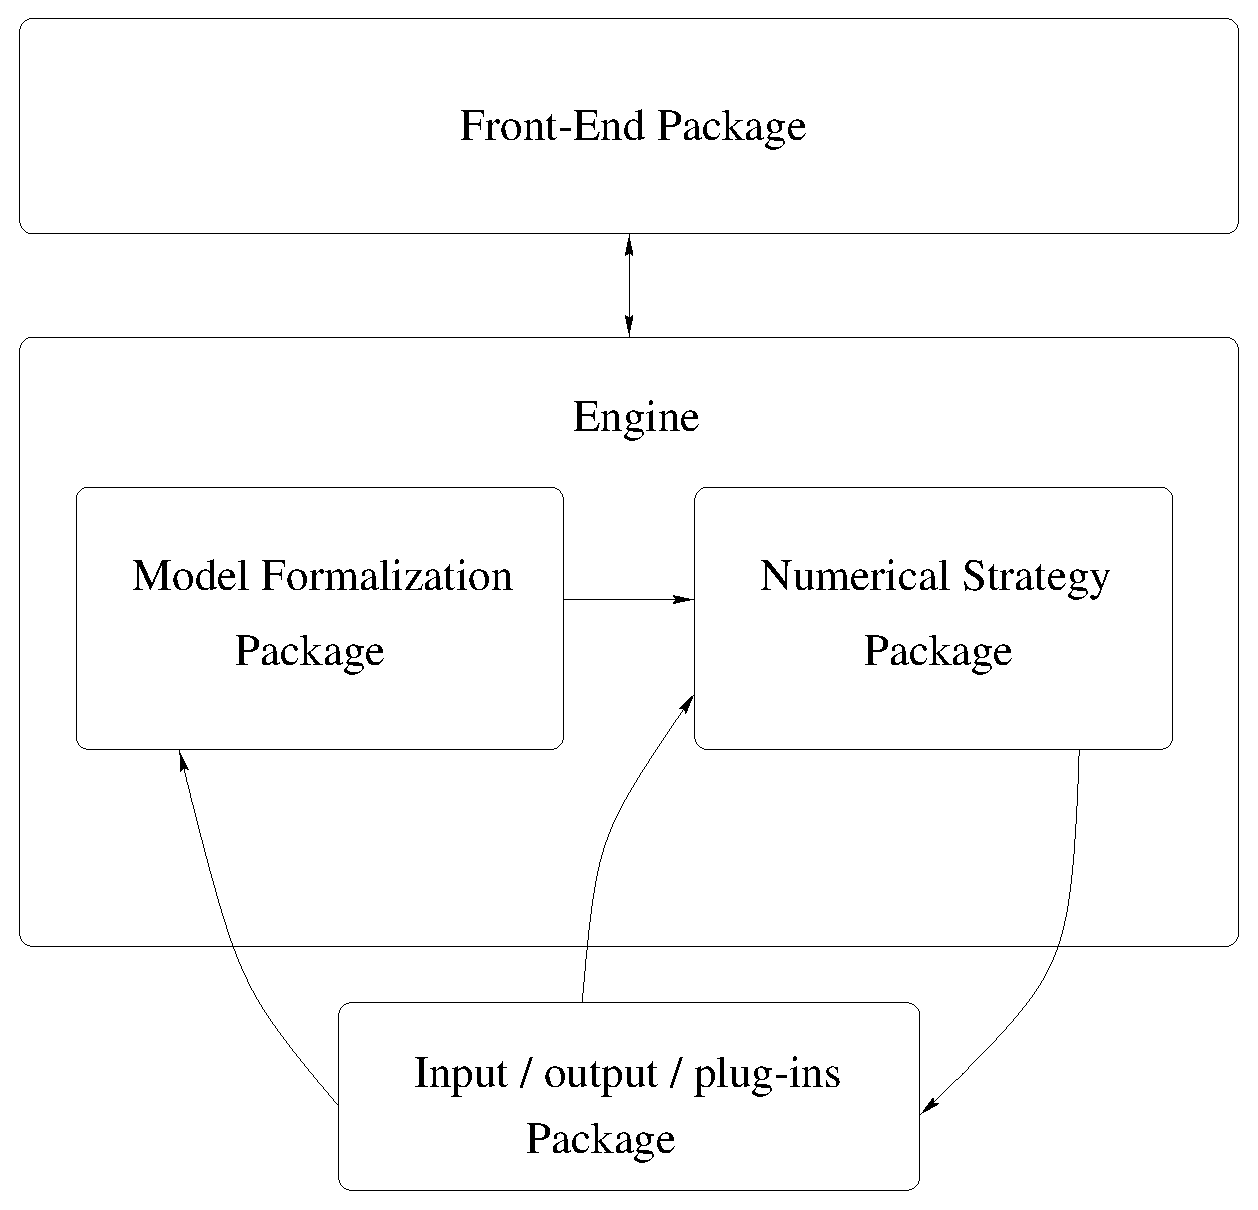
\includegraphics[scale=0.80]{figure/dependency.eps}
\caption{Structure chart of the dependencies}
\label{dependency}
\end{center}
\end{figure}

%\clearpage

The chart \ref{dependency} shows the links seen previously. The Front-end access the platform to drive a complete simulation. The model formalisation uses input methods (basic input method or input method form a dedicated plug-in) to get data, then other
methods to fill the data structure of the platform according to the specificities of each \ac{nsds}.
The numerical strategy uses the model built before to make the computations and an output method (basic output method or output method form a dedicated plug-in) to save the output data.\\

The following diagrams (\ref{sequence_diag1} \& \ref{sequence_diag2}) describe the unfolding of a simulation.
\begin{figure}[!hbp]
\begin{center}
\includegraphics[scale=0.65, bb=30 40 300 775,angle=-90, clip]{figure/sequence1.ps}
\caption{Sequence diagram - Without plug-in}
\label{sequence_diag1}
\end{center}
\end{figure}

\begin{figure}[!hbp]
\begin{center}
\includegraphics[scale=0.65, bb=30 40 330 775,angle=-90, clip]{figure/sequence2.ps}
\caption{Sequence diagram - With plug-in}
\label{sequence_diag2}
\end{center}
\end{figure}

\subsection{Interface view}
We will define in this section the functionalities of the components and their interfaces. 
% It should define the system using one or more of the identity, functions and interface parts of the component description. Suitable methods of presentation are interface files and parameter tables. The intended readership of this description comprises designers, programmers and testers, who need to know how to use the components in the system.
For each communication between components, the information in transit is detailed :
\begin{itemize}

        \item Front-End to Engine\\
        Input files name, matrices, systems, relations that the users want to use for the computations.

        \item Engine to Front-End\\
        Error messages, control messages (``Simulation finished'', indications about the current computation, \dots), some of the simulation result.
        
        \item Model Formalisation to Numerical Strategy\\
        Formalised model, which is composed of several equations (dynamical equation, relations and non smooth laws).
        Most of the equations are composed of matrix.
        
        \item Input/Output/Plug-ins to Model Formalisation\\
        Description of the physical problem. Reading of dedicated files by plug-ins or input/output methods.
        
        \item Plug-ins to Numerical Strategy\\
        Selection of the right methods for computations.
        
        \item Numerical Strategy to Input/Output/Plug-ins\\
        Description of the physical problem at the end or during the simulation.

\end{itemize}

\section{System architecture diagram with related description}
The figure \ref{archi} shows the system architecture using the SA method.
\begin{figure}[p]
\begin{center}
\includegraphics[angle=90, height=22cm]{figure/archi.pstex}
\caption{System architecture - SA diagram}
\label{archi}
\end{center}
\end{figure}
We can see in this figure, the different packages of the architecture.
At first, the package regrouping the input/output modules are represented in light blue and the plug-in modules are represented in dark blue.
In green we see the Front-end package.
In yellow, the Model formalisation package.
In pink, we see the numerical strategy.
Finally, the last module, "update state" is shared between the formalisation and the numerical
strategy package.\\

The diagram \ref{archi_sd} represents the structure we build with the SA diagram. This is the SD diagram.
The one who see is the restructured diagram.
\begin{figure}[p]
\begin{center}
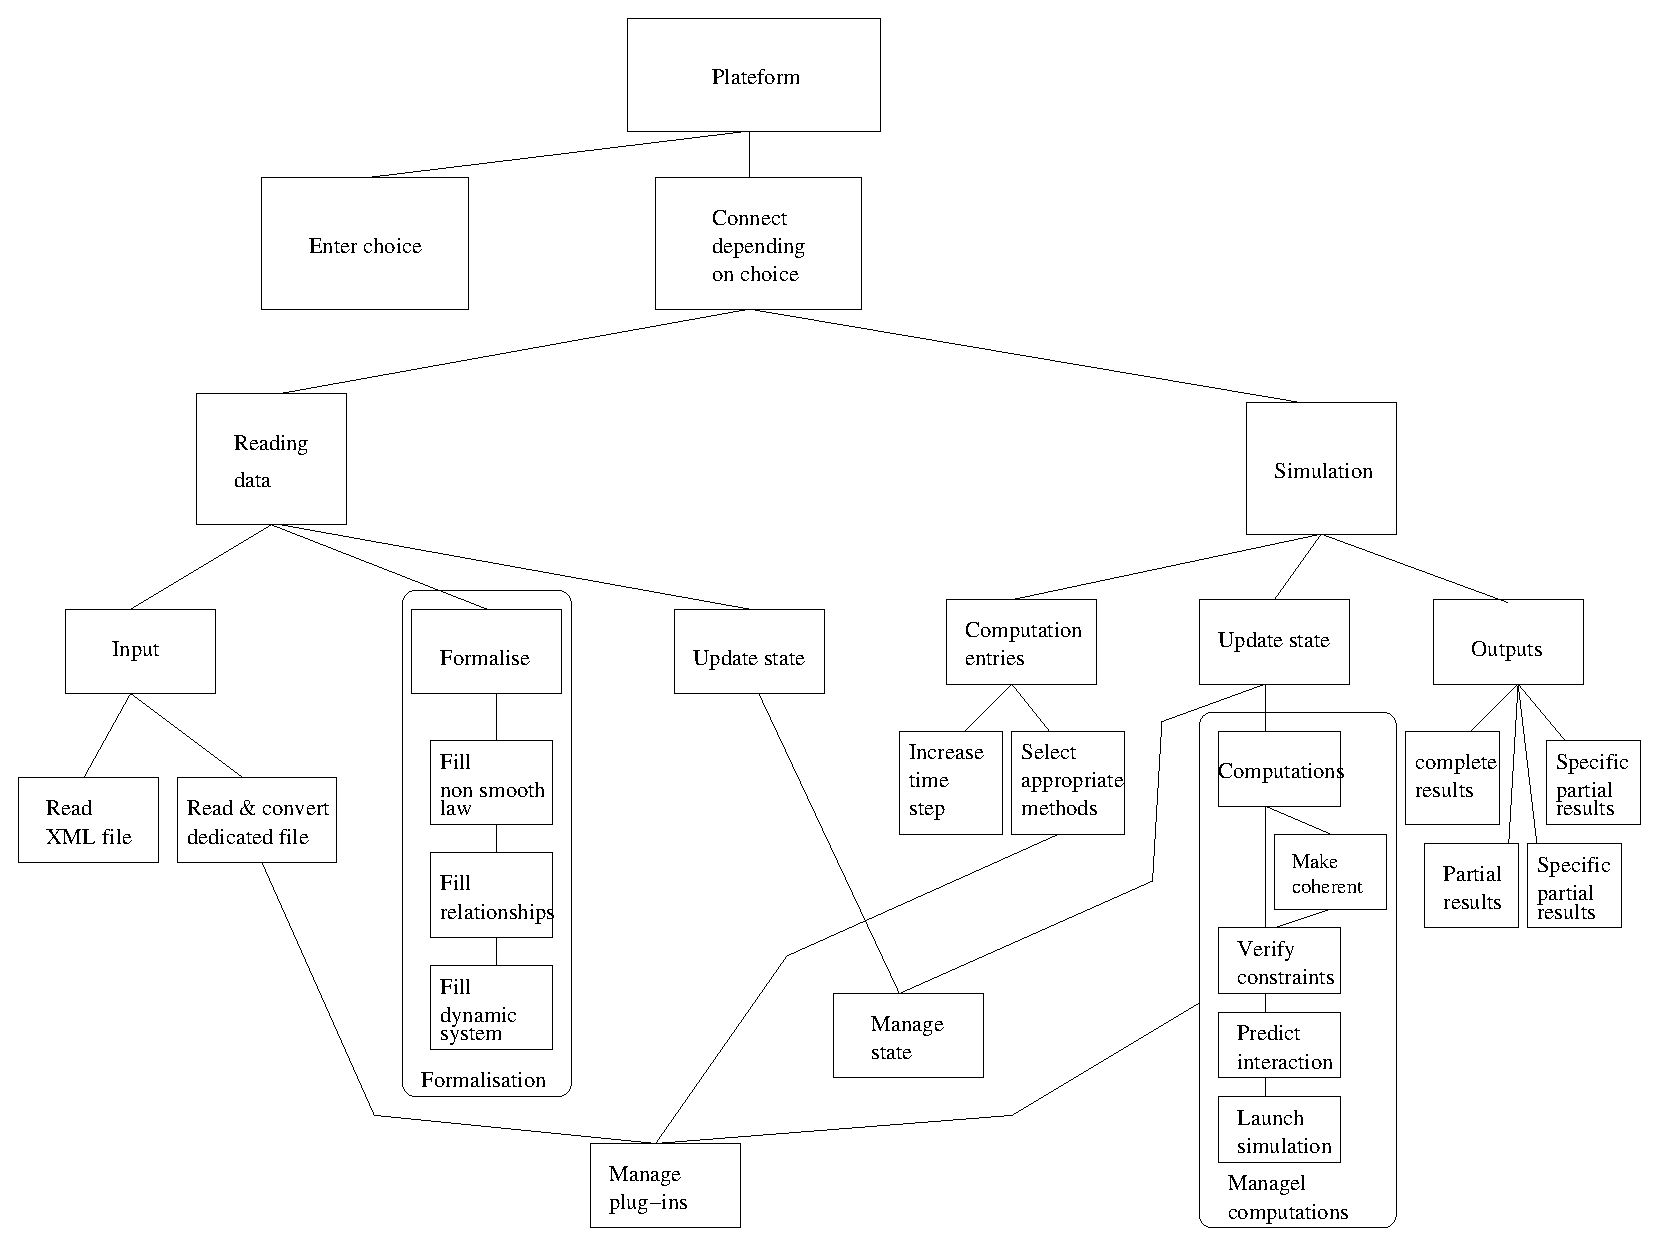
\includegraphics[angle=90, height=22cm]{figure/archi_sd.eps}
\caption{System architecture - SD diagram}
\label{archi_sd}
\end{center}
\end{figure}


\section{SASD conclusion}
The different groups we have made are high cohesion modules because they regroup specific traitments.
During the Detailed Design Phase, we must be carefull with the coupling between these modules.
